\documentclass[12pt,a4paper]{article}
\usepackage[utf8]{inputenc}
\usepackage[catalan]{babel}
\usepackage{graphicx}
\usepackage{geometry}
\usepackage{fancyhdr}
\usepackage{tabularx}
\usepackage{lastpage}
\usepackage{enumitem}
\usepackage{amsmath}
\usepackage{tikz}
\usepackage{tcolorbox}

% 1. MARGES I CAPÇALERA
\geometry{top=3.5cm, bottom=3cm, left=2cm, right=2cm, headheight=2.5cm}

\pagestyle{fancy}
\fancyhf{}
\fancyhead[L]{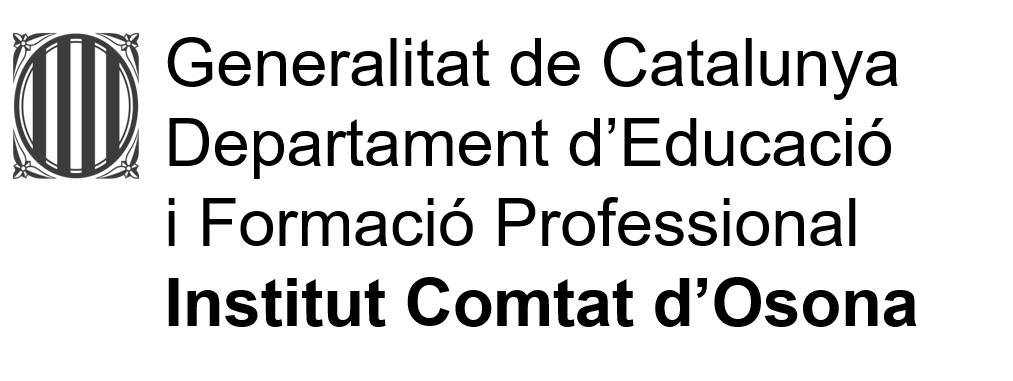
\includegraphics[height=1.8cm]{Logo_Departament.png}} 
\fancyhead[R]{
\includegraphics[height=1.8cm]{Logo_Institut.png}}
\fancyfoot[C]{Pàgina \thepage\ de \pageref{LastPage}}
\renewcommand{\headrulewidth}{0.4pt}

\begin{document}

% --- CAPÇALERA D'IDENTIFICACIÓ ---
\begingroup
\renewcommand{\arraystretch}{2.2}
\begin{tabularx}{\textwidth}{|X|p{4cm}|}
    \hline
    \textbf{Nom i cognoms:} & \textbf{Grup:} \\ \hline
    \textbf{Activitat:} Fitxa de Repàs. Àrees i Perímetres & \textbf{Data:} \\ \hline
\end{tabularx}
\endgroup

\vspace{0.5cm}

\begin{tcolorbox}[colback=gray!5,colframe=gray!80!black,title=\textbf{Conceptes Bàsics}]
    \begin{itemize}[leftmargin=*]
        \item \textbf{Perímetre (P):} És la suma de tots els costats de la figura (el seu contorn). 
        \item \textbf{Àrea (A):} És la superfície que ocupa la figura (el que omple l'interior).
    \end{itemize}
\end{tcolorbox}

\section*{Bloc 1: Quadrilàters (Figures de 4 costats)}

\begin{tcolorbox}[colback=blue!5,colframe=blue!75,title=\textbf{Fórmules per tenir a mà}]
    \textbf{Quadrat:} $A = costat \cdot costat$ \hspace{2cm} \textbf{Rectangle o Romboide:} $A = base \cdot altura$ \\
    \textbf{Rombe:} $A = \frac{D \cdot d}{2}$ \hspace{3.4cm} \textbf{Trapezi:} $A = \frac{(Base_{gran} + base_{petita}) \cdot altura}{2}$
\end{tcolorbox}

\textbf{1. Calcula el perímetre ($P$) i l'àrea ($A$) dels quadrats i rectangles següents.}

\vspace{0.4cm}
\begin{tabularx}{\textwidth}{@{} X X @{}}
    a) Quadrat de $5\text{ cm}$ de costat. & b) Rectangle de base $8\text{ cm}$ i altura $3\text{ cm}$. \\
    \begin{tikzpicture}[scale=0.5]
        \draw[thick, fill=blue!10] (0,0) rectangle (3,3);
        \node at (1.5,-0.6) {$5\text{ cm}$};
        \node at (-0.8,1.5) {$5\text{ cm}$};
    \end{tikzpicture} & 
    \begin{tikzpicture}[scale=0.5]
        \draw[thick, fill=blue!10] (0,0) rectangle (6,2.5);
        \node at (3,-0.6) {$8\text{ cm}$};
        \node at (7,1.25) {$3\text{ cm}$};
    \end{tikzpicture} \\[0.2cm]
    $P = $ & $P=$ \\
    $A = $ & $A=$\\[0.6cm]
    
    c) Quadrat de $10\text{ m}$ de costat. & d) Rectangle de base $12\text{ m}$ i altura $5\text{ m}$. \\
    $P = $ & $P=$ \\
    $A = $ & $A=$\\[0.6cm]
\end{tabularx}

\textbf{Anota el aprenentatges al diari d'aula}

\newpage

\section*{Bloc 2: L'Àrea dels Triangles}

\begin{tcolorbox}[colback=green!5,colframe=green!75,title=\textbf{Atenció amb el triangle!}]
    En qualsevol triangle, l'àrea sempre és la meitat d'un rectangle: \quad $\mathbf{A = \frac{base \cdot altura}{2}}$
\end{tcolorbox}

\textbf{3. Calcula l'àrea d'aquests triangles. Identifica bé quina és la base i l'altura.}

\vspace{0.5cm}
\begin{tabularx}{\textwidth}{@{} X X @{}}
    a) Triangle rectangle & b) Triangle isòsceles \\
    \begin{tikzpicture}[scale=0.6]
        \draw[thick, fill=green!10] (0,0) -- (5,0) -- (0,4) -- cycle;
        \draw (0.3,0) -- (0.3,0.3) -- (0,0.3);
        \node at (2.5,-0.5) {$base = 6\text{ cm}$};
        \node at (-1.4,2) {$altura = 4\text{ cm}$};
    \end{tikzpicture} & 
    \begin{tikzpicture}[scale=0.6]
        \draw[thick, fill=green!10] (0,0) -- (6,0) -- (3,4) -- cycle;
        \draw[dashed] (3,0) -- (3,4) node[midway,right]{$5\text{ m}$};
        \draw (3.3,0) -- (3.3,0.3) -- (3,0.3);
        \node at (3,-0.5) {$base = 8\text{ m}$};
    \end{tikzpicture} \\[0.2cm]
    $A = \dfrac{\dots \cdot \dots}{2} = \dots\dots\dots$ & $A = \dfrac{\dots \cdot \dots}{2} = \dots\dots\dots$ \\[0.8cm]
    
    c) $base = 10\text{ cm}$, $altura = 7\text{ cm}$. & d) $base = 20\text{ m}$, $altura = 15\text{ m}$. \\
    $A = \makebox[4cm]{\hrulefill}$ & $A = \makebox[4cm]{\hrulefill}$ \\
\end{tabularx}
\vspace{0.3cm}
\textbf{Anota els aprenentatges al diari d'aula}
\vspace{0.8cm}

\section*{Bloc 3: El Cercle i la Circumferència}

\begin{tcolorbox}[colback=red!5,colframe=red!75,title=\textbf{Les fórmules rodones} (Fes servir $\pi = 3,14$)]
    \textbf{Longitud} (és com el perímetre): $L = 2 \cdot \pi \cdot radi$ \\
    \textbf{Àrea} (el que ocupa a dins): $A = \pi \cdot radi^2$ 
\end{tcolorbox}


\textbf{4. Troba la Longitud ($L$) i l'Àrea ($A$) d'aquests cercles.}

\vspace{0.4cm}
\begin{tabularx}{\textwidth}{@{} X X @{}}
    a) Cercle de radi $r = 3\text{ cm}$. & b) Cercle de radi $r = 10\text{ m}$. \\
    \begin{tikzpicture}[scale=0.8]
        \draw[thick, fill=red!10] (0,0) circle (2);
        \draw[thick,->] (0,0) -- (2,0) node[midway,above]{$3\text{ cm}$};
        \filldraw (0,0) circle (1.5pt);
    \end{tikzpicture} & 
    \begin{tikzpicture}[scale=0.8]
        \draw[thick, fill=red!10] (0,0) circle (2);
        \draw[thick,->] (0,0) -- (1.41,1.41) node[midway,above left]{$10\text{ m}$};
        \filldraw (0,0) circle (1.5pt);
    \end{tikzpicture} \\[0.2cm]
    $L = 2 \cdot 3,14 \cdot \dots = \dots\dots\dots$ & $L = 2 \cdot 3,14 \cdot \dots = \dots\dots\dots$ \\
    $A = 3,14 \cdot \dots^2 = \dots\dots\dots$ & $A = 3,14 \cdot \dots^2 = \dots\dots\dots$ \\
\end{tabularx}

\vspace{0.3cm}
\textbf{Anota els aprenentatges al diari d'aula}
\end{document}